%%%%%%%%%%%%%%%%%%%%%%%%%%%%%%%%%%%%%%%%%%%%%%%%%%%%%%%%%%%%%%%%%%%%%%%%%%%%%%%%
%
%  Project: IsaNet
%
%  Module:  document/root.tex (Isabelle/HOL 2021)
%  Author:  Tobias Klenze / Christoph Sprenger
%  
%  root file for generation of PDF document
%
%  Copyright (c) Tobias Klenze / Christoph Sprenger 
%  Licence: LGPL
%
%%%%%%%%%%%%%%%%%%%%%%%%%%%%%%%%%%%%%%%%%%%%%%%%%%%%%%%%%%%%%%%%%%%%%%%%%%%%%%%%

\documentclass[11pt,a4paper]{report}
\usepackage{isabelle,isabellesym}

% additional packages
\usepackage{graphicx}       % to display session graph
\usepackage{a4wide}
\usepackage{verbatim}
% have each section start on a fresh page
\renewcommand{\isamarkupsection}[1]{\newpage\section{#1}}

% this should be the last package used
\usepackage{pdfsetup}

% for special symbols 
\usepackage{amssymb}

% urls in roman style, theory text in math-similar italics
\urlstyle{rm}
\isabellestyle{it}


\begin{document}


\title{IsaNet: Formalization of a Verification Framework for Secure Data Plane Protocols}
\author{Tobias Klenze, Christoph Sprenger}
\maketitle

\tableofcontents

\newpage

The paper presenting this formalization is to appear in the Journal of Computer Security under the title ``IsaNet: A Framework for Verifying Secure Data Plane Protocols''.

This is a generated file containing all of our models, from abstract to parametrized to protocol instances, that we formalized in Isabelle/HOL in a human-readable form. 
The theory dependencies given in the figure on the next page are useful.
Nevertheless, the most convenient way of browsing the Isabelle theories is to use the GUI shipped with Isabelle. See the README for details.

\textbf{Abstract (from JCS paper)}

Today's Internet is built on decades-old networking protocols that lack scalability, reliability and security.
In response, the networking community has developed \emph{path-aware} Internet architectures that solve these issues while simultaneously empowering end hosts.
In these architectures, autonomous systems authorize forwarding paths in accordance with their routing policies, and protect paths using cryptographic authenticators.
For each packet, the sending end host selects an authorized path and embeds it and its authenticators in the packet header. This allows routers to efficiently determine how to forward the packet.
The central security property of the data plane, i.e., of forwarding, is that packets can only travel along authorized paths. This property, which we call \emph{path authorization}, protects the routing policies of autonomous systems from malicious senders.

The fundamental role of packet forwarding in the Internet's ecosystem and the complexity of the authentication mechanisms employed call for a formal analysis.
We develop IsaNet, a parameterized verification framework for data plane protocols in Isabelle/HOL. We first formulate an abstract model without an attacker for which we prove path authorization. We then refine this model by introducing a Dolev--Yao attacker and by protecting authorized paths using (generic) cryptographic validation fields. This model is parametrized by the path authorization mechanism and assumes five simple verification conditions.
We propose novel attacker models and different sets of assumptions on the underlying routing protocol.
We validate our framework by instantiating it with nine concrete protocols variants and prove that they each satisfy the verification conditions (and hence path authorization). 
The invariants needed for the security proof are proven in the parametrized model instead of the instance models. Our framework thus supports low-effort security proofs for data plane protocols. 
In contrast to what could be achieved with state-of-the-art automated protocol verifiers, our results hold for arbitrary network topologies and sets of authorized paths.


% sane default for proof documents
\parindent 0pt\parskip 0.5ex

% display the theory dependency graph
%%%%%%%%%%%%%%%%%%%%%%%%%%%%%%%%%%%%%%%%%%%%%%%%%%%%%%%%%%%%%%%%%%%%%%%%%%%%%%%%
%
%  Project: Sumcheck Protocol 
%
%  Authors:  Azucena Garvia <zucegb@gmail.com>
%		   Christoph Sprenger <sprenger@inf.ethz.ch>
%		   Jonathan Bootle <jbt@zurich.ibm.com>
%  
%%%%%%%%%%%%%%%%%%%%%%%%%%%%%%%%%%%%%%%%%%%%%%%%%%%%%%%%%%%%%%%%%%%%%%%%%%%%%%%%

\begin{figure}[p]
  \begin{center}
    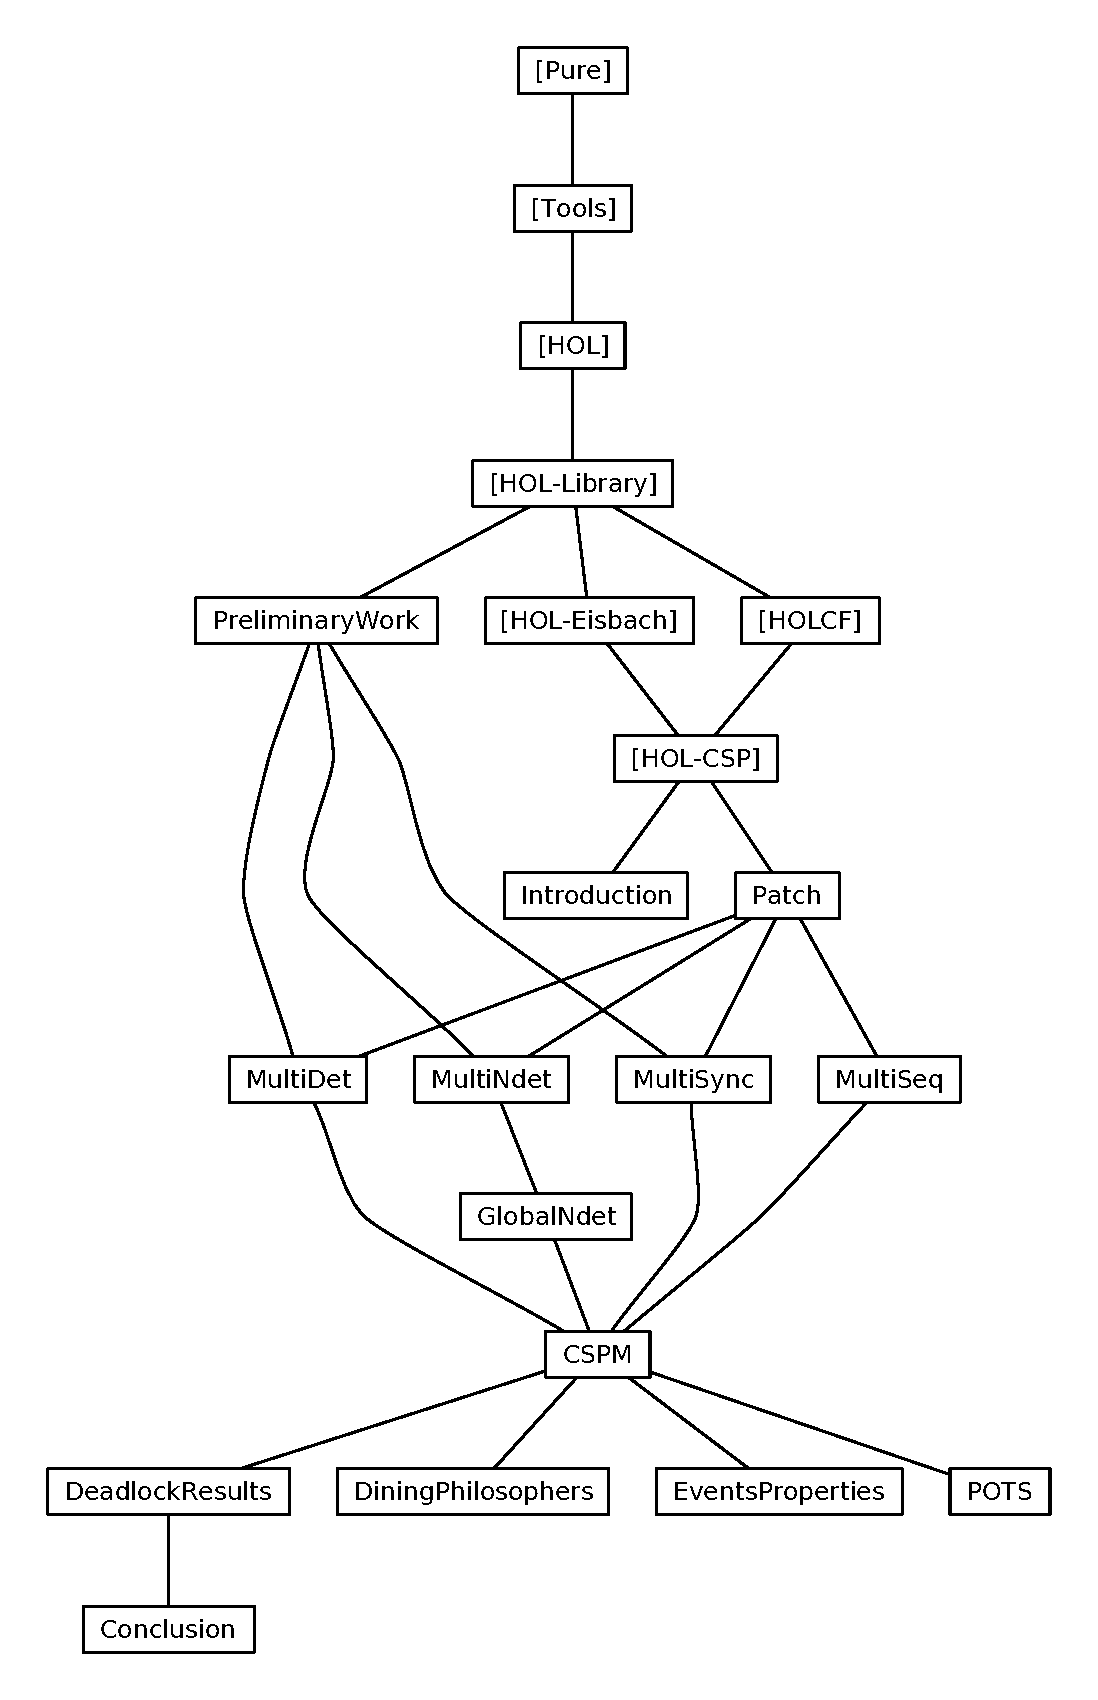
\includegraphics[scale=.7]{session_graph.pdf}
    \caption{Theory dependencies}
  \end{center}
  \label{fig:theory-dependencies}
\end{figure}



% generated text of all theories
\input{session}

% optional bibliography
%\bibliographystyle{abbrv}
%\bibliography{root}

\end{document}

